%%%%%%%%%%%%%%%%%%%%%%%%%%%%%%%%%%%%%%%%%
% University Assignment Title Page 
% LaTeX Template
% Version 1.0 (27/12/12)
%
% This template has been downloaded from:
% http://www.LaTeXTemplates.com
%
% Original author:
% WikiBooks (http://en.wikibooks.org/wiki/LaTeX/Title_Creation)
%
% License:
% CC BY-NC-SA 3.0 (http://creativecommons.org/licenses/by-nc-sa/3.0/)
% 
% Instructions for using this template:
% This title page is capable of being compiled as is. This is not useful for 
% including it in another document. To do this, you have two options: 
%
% 1) Copy/paste everything between \begin{document} and \end{document} 
% starting at \begin{titlepage} and paste this into another LaTeX file where you 
% want your title page.
% OR
% 2) Remove everything outside the \begin{titlepage} and \end{titlepage} and 
% move this file to the same directory as the LaTeX file you wish to add it to. 
% Then add \input{./title_page_1.tex} to your LaTeX file where you want your
% title page.
%
%%%%%%%%%%%%%%%%%%%%%%%%%%%%%%%%%%%%%%%%%
%\title{Title page with logo}
%----------------------------------------------------------------------------------------
%	PACKAGES AND OTHER DOCUMENT CONFIGURATIONS
%----------------------------------------------------------------------------------------

\documentclass[12pt]{report}
\usepackage[english]{babel}
\usepackage{apacite}
\usepackage{array,etoolbox}
\preto\tabular{\setcounter{magicrownumbers}{0}}
\newcounter{magicrownumbers}
\usepackage[utf8x]{inputenc}
\usepackage{geometry}
	\geometry{
		a4paper,
		total = {160mm, 245mm},
		left = 30mm,
		top = 30mm
	}
\usepackage[super,sort]{natbib}
\usepackage{tgbonum}
\usepackage{amsmath}
\usepackage{graphicx}
\graphicspath{{images/}}
\usepackage[colorinlistoftodos]{todonotes}
\usepackage{amsmath}

\begin{document}

\begin{titlepage}

\newcommand{\HRule}{\rule{\linewidth}{0.5mm}} % Defines a new command for the horizontal lines, change thickness here

\center % Center everything on the page
 
%----------------------------------------------------------------------------------------
%	HEADING SECTIONS
%----------------------------------------------------------------------------------------

\textsc{\LARGE Northeastern University}\\[1.5cm] % Name of your university/college
\textsc{\Large Master's Thesis Proposal}\\[0.5cm] % Major heading such as course name
\textsc{\large CS 7990}\\[0.5cm] % Minor heading such as course title

%----------------------------------------------------------------------------------------
%	TITLE SECTION
%----------------------------------------------------------------------------------------

\HRule \\[0.4cm]
{\Large \bfseries Word-vector Regularization for text classification algorithms}\\[0.4cm] % Title of your document
\HRule \\[1.5cm]
 
%----------------------------------------------------------------------------------------
%	AUTHOR SECTION
%----------------------------------------------------------------------------------------

\begin{minipage}{0.4\textwidth}
\begin{flushleft} \large
\emph{Author:}\\
Ramkishan \textsc{Panthena} % Your name
\end{flushleft}
\end{minipage}
~
\begin{minipage}{0.4\textwidth}
\begin{flushright} \large
\emph{Advisor:} \\
Dr. Virgil \textsc{Pavlu} % Supervisor's Name
\end{flushright}
\end{minipage}\\[.5cm]

\begin{minipage}{0.82\textwidth}
\begin{flushright} \large
\emph{Official Reader:} \\
Dr. Byron \textsc{Wallace} % Reader's Name
\end{flushright}
\end{minipage}\\[2cm]

% If you don't want a supervisor, uncomment the two lines below and remove the section above
%\Large \emph{Author:}\\
%John \textsc{Smith}\\[3cm] % Your name

%----------------------------------------------------------------------------------------
%	DATE SECTION
%----------------------------------------------------------------------------------------

{\large \today}\\[2cm] % Date, change the \today to a set date if you want to be precise

%----------------------------------------------------------------------------------------
%	LOGO SECTION
%----------------------------------------------------------------------------------------


\includegraphics[width=4cm, height=4cm]{logo.jpg}\\[1cm] % Include a department/university logo - this will require the graphicx package
 
%----------------------------------------------------------------------------------------

%\vfill % Fill the rest of the page with whitespace

\end{titlepage}

\begin{abstract}
A simple and efficient baseline for text classification is to represent sentences as bag-of-words (BoW) and train a linear classifier. The bag-of-words model is simple to implement and offers flexibility for customization by providing different scoring techniques for user specific text data. In many problem domains, these linear classifiers are preferred over more complex models like CNN, LSTM because of their efficiency, robustness and interpretability.

However, a large vocabulary can cause extremely sparse representations which are harder to model, where the challenge is for models to harness very little information in such a large representational space. Also, these classification problems are categorized by large number of classes and highly imbalanced distribution of data across these classes. In such cases, the traditional linear classifiers would treat each word separately and assign them different coefficients based on the frequency in which they occur in the train set. This would result in lower test accuracy when it comes across instances where a word which was occurring less frequently in the train set, occurs more often in the test set.

Our thesis aims to solve this problem by constraining weights of rare features by similar, more frequent ones, using semantic similarity. This would enforce similar words to have similar weights thereby improving model performance. Thus, based on how similar two features are, our proposed model can improve the feature importance of a sparse word by increasing its regression co-efficient, thereby improving the test accuracy in the above mentioned scenario.

\end{abstract}

\section{Introduction}

The goal of text classification is to classify text documents into one or more classes according to their content. For this purpose, a document must be transformed into a representation which is suitable for the learning algorithm and the classification task. Representing documents as bag-of-words is a commonly used method in document classification where the frequency of occurrence of each word is used as a feature for training a classifier. However, one should note that when using this representation, some document information is lost as the model disregards grammar and word ordering.

\subsection{Problem Statement}

Although the bag-of-words model is widely used and performs exceptionally well in most text classification problems, it contains several limitations. As per Zipf's law \cite{li1992random}, given a large sample of words used, the frequency of any word is inversely proportional to its rank in the frequency table. So, word number n has a frequency proportional to 1/n. Thus, a large vocabulary can cause extremely sparse representations. 

The classification accuracy we observe on the test set largely depends on the quality of training sets we have used to build our models. That is, if the training information is sparse, then we can expect the category model to be a poor representation of a category thereby leading to poor classification accuracy. Words that occur rarely do not give a learning algorithm enough information to determine its influence on classification correctly.

Thus, in such a case any linear classifier like logistic regression, naive bayes, linear SVM would treat each word independently and assign them different coefficients based on the impact of the individual word on the response variable. As the training data for rare words would be sparse, their coefficients would be near 0 implying that the impact of these features is small. This may not be the case as these rare words might be misrepresented due to sparse data. Our model tries to solve this problem by using a word-vector regularizer that assigns similar coefficients to words which are used in a similar context, thereby boosting the effect of similar but rare features on the final prediction.

We use logistic regression for binary text classification on a bag-of-words model. Let $\theta^{(i)}$ be the regression coefficients of word$_{i}$ which determines the association between each feature value (word occurrence in document) and what the target we are trying to predict.

\noindent The cost function for logistic regression would be given as:

\begin{equation}\label{lr_cost_fn_eq}
Cost(h_{(\theta)}(x), y) = 
\begin{cases}
-log(h_{(\theta)}(x)), $\qquad if y=1$
\\
-log(1-h_{(\theta)}(x)), $ if y=0$
\end{cases}
\end{equation}\\

In general, the features with larger coefficients are more important because they make a significant contribution in predicting the correct class. However if a word$_{k}$ is rare, its corresponding regression coefficient ($\theta^{(k)}$) could be very small or very large (minimizing the loss) due to lack of evidence in the training set; which is not useful for predictions. Our plan here is to constrain such coefficients by the word semantic similarity with other more frequent terms, thus simulating a higher occurence and prohibiting extreme behavior. This also helps with non-frequent synonym words in making their coefficients more uniform. \\

\noindent \textbf{Example:} In order to get a better understanding, consider a classification problem where we are trying to identify whether a document is talking about animals or not. For this example, let's say we only have five features. The bag-of-words representation using term frequencies for 5 different documents would look like:

\begin{table}[htbp]
\centering
\begin{tabular}{l|lllll}
 & dog & \multicolumn{1}{c}{football} & \multicolumn{1}{c}{canine} & movies & cat \\\hline
D1 & 3 & 0 & 0 & 0 & 4 \\
D2 & 0 & 0 & 0 & 6 & 0 \\
D3 & 5 & 0 & 1 & 0 & 6 \\
D4 & 0 & 8 & 0 & 0 & 0 \\
D5 & 0 & 7 & 0 & 4 & 0
\end{tabular}
\caption{Toy dataset}
\end{table}

From the above example, we can see that the word ‘canine’ occurs only once in one of the document. If we train a linear classifier on the above dataset, then ‘canine’ would have a very low feature importance due to its sparse representation. When we test this classifier on a document where ‘canine’ is more densely represented as compared to ‘dog’ or ‘cat’, then that document would get misclassified as “not talking about animals”. 

In contrast, since our model would assign similar weights to similar words and considering ‘dog’ and ‘canine’ are synonyms, our model would assign a higher feature importance to ‘canine’, thereby increasing the probability of making a correct prediction on a new document where ‘canine’ is more densely represented as compared to the train data.


\chapter{Related work}

A number of approaches have been proposed to increase the classification accuracy on the bag-of-words model.

To aggressively reduce the dimensionality of models, Joachims \cite{joachims1996probabilistic} (1996), Yang and Pedersen\cite{yang1997comparative} (1997) suggested pruning of infrequent words. Mansuy and Hilder \cite{mansuy2006characterization} (2006) recommended removing of stop words and part-of-speech tags. Porter \cite{porter1980algorithm} (1980) proposed removal of suffixes from words. However, Joachims \cite{joachims1996probabilistic} test results revealed that the performance of the system is higher when more words are used as features, with the highest performance achieved using the largest feature set. Any approach that limited the number of words to the most important ones was likely to reduce the classification accuracy as these pruned words lose their ability to contribute to the classification of text. Quinlan \cite{quinlan2014c4} (1993) suggested choosing words which have high mutual information with the target concept. However, picking words with high mutual information had relatively poor performance due to its bias towards favoring rare terms, and its sensitivity to probability estimation errors.

In an attempt to address the issue of related concepts in text classification, many researchers have incorporated features using dictionaries and encyclopedias. Mavroeidis et. al \cite{mavroeidis2005word} (2005) proposed to extend the traditional bag of words representation by incorporating syntactic and semantic relationships among words using a Word Sense Disambiguation approach. Wang and Domeniconi \cite{wang2008building} (2008) explored a similar approach by embedding background knowledge derived from Wikipedia to enrich the representation of documents. Although empirical results have shown improvements in some cases, the applicability of using dictionaries to improve classification accuracy is limited. Ontology is manually built, and the coverage is far too restricted. Recently, Heal et. al \cite{heap2017word} (2017) introduced a method for enriching the bag-of-words model by complementing rare term information with related terms from Word Vector models. However, it was revealed that these methods achieved significantly better results only when the training sets were small. There wasn't enough evidence of achieving better results on large datasets.

In addition to incorporating related concepts to improve classification performance, other approaches have also been proposed. One of these approaches considers using part-of-speech tags associated with words contained in a document (Scott and Matwin \cite{scott1998text} 1998), (Jensen and Martinez \cite{jensen2000improving} 2000). Since words can have multiple meanings depending upon how and where they are used in a sentence, the part-of-speech may be relevant to text classification. However, a different paper from Mansuy \cite{mansuy2006characterization} revealed that there was no significant difference between the accuracy of the classifiers whether part-of-speech tags are utilized or not.

To deal with overfitting, different regularization techniques have also been proposed. Regularization adds a penalty on the different parameters of the model to reduce the freedom of the model. Hence, the model will be less likely to fit the noise and improve its generalization abilities. The Lasso regularization acts as a way of feature selection by shrinking some parameters to zero, whereas the Ridge regularization will force the parameters to be relatively small but are not cut to zero.

\chapter{Proposed Method}

In this method, we propose to enhance the bag-of-words model for text classification by presenting a novel regularizer which would assign similar coefficients to words used in similar context.

\begin{figure}
\centering
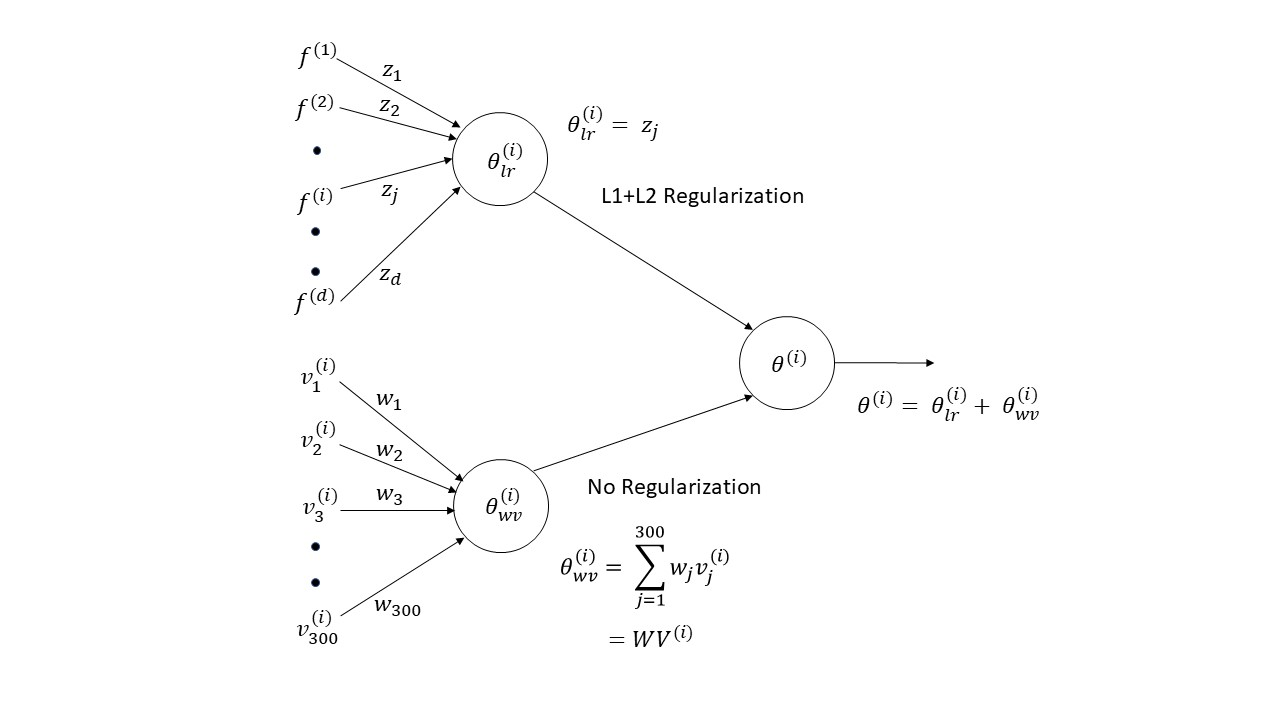
\includegraphics[width=18cm, height=10cm]{images/Fig3.jpg}\\
\centering
\caption{Network diagram to learn $\theta^{(i)}$ from word$_{i}$ representation f(v$^{(i)}$)}
\label{fig:foo}
\end{figure}

Formally, the problem we are trying to solve can be formulated as follows: Given a set of m documents with n features, the documents would be represented by matrix X $\in$ R$^{m x n}$. We want to find the coefficients that predict the output Y from the documents X and we want to build a model where the coefficients ($\theta^{(i)}$) are a function of its word$_{i}$ representation ($v^{(i)}$), i.e.,

\begin{equation}\label{lb1}
\theta^{(i)} = f(v^{(i)})
\end{equation}

This would act as a regularization constraint so that similar word representations would have similar coefficients, which satisfies a continuity condition

\begin{equation}
|f(v^{(1)}) - f(v^{(2)}))|\ \leq\ sim(v^{(1)}, v^{(2)})
\end{equation}

where, $sim$ dictates the similarity between words $v^{(1)}$ and $v^{(2)}$ and $ f(v^{(1)}), f(v^{(2)})$ are coefficients of their respective words as per (\ref{lb1})

% $\quad\qquad\ \epsilon $ is the smallest constant satisfying the equation (Lipschitz constant)\\

Since words used in similar context will have similar word-vectors and by making the regression co-efficient of a word to be a function of its word-vector representation, we can regularize the regression coefficients of two similar words to have similar values. So, if one word occurs more frequently and has higher regression co-efficient, the other word even if it is very rare would be considered an important feature and would have a higher regression co-efficient. This would improve the classification performance in cases where these rare words occur more frequently in the test set.\\

% Our goal is to regularize the text classifier coefficients using word-vectors. However, for the thesis our objective is to learn the function $f(v^{(i)})$ and use it to regularize regression on text. \\


\noindent We explore learning the function $f(v^{(i)})$ via several algorithms:

\begin{itemize}
\item regression
\item 2-layer neural network
\item boosting trees
\end{itemize}

\noindent Fig. 1 is a network diagram showing how the coefficients ($\theta_{i}$) would be obtained for a word$_{i}$ representation using both the above mentioned methods.\\
%%%%%%%%%%%%%%%%%%%%%%%%%%%%%%%%%%
\noindent\textbf{Learning f as Regression}: We will initially determine if we can learn the coefficients from the word representation of the features using a linear regressor, i.e., 

\begin{equation}
\theta^{(i)} = w_{1}v_{1}^{(i)} + w_{2}v_{2}^{(i)} + ... + w_{d}v_{d}^{(i)} = \sum_{d=1}^{D} w_{d}^{(i)}v_{d}^{(i)}
\end{equation}

where, $w = (w_{1}, w_{2}, ..., w_{d}$) are the parameters of the regression function. 

$\quad\qquad\  v= (v_{1}, v_{2}, ..., v_{d})$ are d-dimensional word-representations of word $i$\\

Within the class of linear functions, our task shall be to find the best parameters $w$ that minimize the error function such that,

\begin{equation}\label{cost_fn_eq}
Cost(h_{(\theta| w)}(x), y) = 
\begin{cases}
-log(h_{(\theta| w)}(x)), $\qquad if y=1$
\\
-log(1-h_{(\theta| w)}(x)), $ if y=0$
\end{cases}
\end{equation}\\
%%%%%%%%%%%%%%%%%%%%%%%%%%%%%%%%%%
\noindent\textbf{Learning f as 2-layer neural network}: If there is a non-linear relationship between the coefficients and word representations, we can learn them through a multi-layer neural network. We start with a 2-layer neural network having one hidden layer and one output layer. The hidden layer requires the d-dimensional word$_{i}$ representations as input and outputs an activation value.\\\\ Let $a^{[1](i)} = (a^{[1](i)}_{1},a^{[1](i)}_{2},a^{[1](i)}_{3}..)$ be the activation of the neurons in the hidden layer, and $a^{[2](i)}$ be the activation of the neurons in the output layer.\\

\noindent where, a = g(z), where g is some activation function (like sigmoid, relu, tanh)

\quad\quad z = Wx + b, where x are the features from the input layer

\quad\quad a$^{[l]}_{k}$ denotes the activation of the $k^{th}$ unit in layer $l$

\quad\quad $x^{(i)}$ with parenthesis refers to the i$^{th}$ word

\quad\quad a$^{[1]}$ is the concatenation of all first layer activations\\

\noindent For a 2-layer neural network, we would have the following parameters:

\begin{alignat}{2}
z^{[1](i)} & = W^{[1]}V^{(i)} + b^{[1]}\\
a^{[1](i)} & = g(z^{[1](i)})\\
z^{[2](i)} & = W^{[2]}a^{[1](i)} + b^{[2]}\\
\theta^{(i)} & = a^{[2](i)} = g(z^{[2]})
\end{alignat}

\noindent We can then train a neural network model to learn the coefficients ($\theta^{(i)}$) which would help minimize the cost function in (\ref{cost_fn_eq})

% \section{Implementation}

\subsection{Obtain word-vectors}

Out of the successful deep learning models used for word-embeddings, two of the most popular ones are Word2Vec \cite{le2014distributed} and Global Vectors \cite{pennington2014glove}. For our research, we will be using Google's Word2Vec which has pre-trained word-vectors with 300 dimensions trained using over 100 billion words. 

Also it has been seen that a smaller domain specific Word Vector model is modelled better than a general model trained over a much larger corpus of text. Thus Google's pre-trained Word Vector model which was trained over three million unique words and phrases will be retrained on the training data to generate domain specific Word Vectors.

\subsection{Train new model}

Once the features have been extracted using the bag-of-words model and their corresponding word-vectors obtained, we can train a neural network model based on the cost function in (\ref{cost_fn_eq})\\

\noindent Below is the link to its source code on GitHub. It will be made publicly available upon thesis completion:

\noindent \url{https://github.com/RamkishanPanthena/Master-s-Thesis}

\newpage
\section{Experiments}

% \section{Baseline}

We compare our model to the vanilla logistic regression algorithm by implementing both using the TensorFlow library. Both the models can perform multi-class and multi-label classification. For multi-class, we use the softmax function to assign probabilities to each class which add up to 1. We use the sigmoid function for multi-label classification to train an independent logistic regression model for each class and accept all labels greater than a certain threshold as predictions.

We tune our model using learning rate and regularization parameter as hyper-parameters and train with different number of epochs till the loss converges. For multi-label problems, we also use prediction threshold as one of the hyper-parameters to list labels with probabilities greater than the threshold value.

\subsection{Evaluation}

To evaluate the performance of both models for multi-class problems, we use accuracy and F1 measures.

For multi-label problems, predictions for an instance is a set of labels, and therefore the prediction can be fully correct, partially-correct or fully-incorrect. Thus, to better evaluate our models we will use the following three measures: \textit{set accuracy}, which is the ratio of perfectly matched instances to the total number of instances; \textit{instance-F1}, which evaluates the performance of partially correct predictions averaged over instances; \textit{label-F1}, which evaluates the performance of partially correct predictions averaged over labels.\\

For a dataset with ground truth labels $y^{(n)}$ and predictions $\hat{y}^{(n)}$, and n instances where n = 1,2,...,N, these three measures are defined as:

\begin{alignat}{2}
set\; accuracy & = \frac{1}{N} \sum_{n=1}^{N} {I(y^{(n)} = \hat{y}^{(n)})}\\
instance \mbox{-} F1 & = \frac{1}{N} \sum_{n=1}^{N} \frac{2\sum_{l=1}^{L} {y^{(n)}_{l} \hat{y}^{(n)}_{l}}}{\sum_{l=1}^{L} {y^{(n)}_{l}} + \sum_{l=1}^{L} {\hat{y}^{(n)}_{l}}}
\hspace{6ex}
label \mbox{-} F1 & = \frac{1}{N} \sum_{n=1}^{N} \frac{2\sum_{n=1}^{N} {y^{(n)}_{l} \hat{y}^{(n)}_{l}}}{\sum_{n=1}^{N} {y^{(n)}_{l}} + \sum_{n=1}^{N} {\hat{y}^{(n)}_{l}}}
\end{alignat}

\noindent where for each instance $n$, $y^{(n)}_{l}$ = 1 if label $l$ is a given label in ground truth; \\
$\hat{y}^{(n)}_{l}$ = 1 if label $l$ is a predicted label.
\newpage
\subsection{Datasets}

\subsubsection{IMDb}

The IMDb dataset is created by Meka with movie plot text summaries labelled with genres sourced from the Internet Movie Database Interface. It is a collection of 35,000 documents partitioned across 25 different genres. The task is to assign multiple genres to a movie description.

Below is a list of the 25 different genres with individual genre counts.

\begin{table}[htbp]
\begin{tabular}{ll|ll}
Drama       & 11726 & Family    & 1564 \\
Comedy      & 7279  & Biography & 1151 \\
Romance     & 4488  & War       & 1049 \\
Thriller    & 4468  & Animation & 949  \\
Crime       & 3195  & History   & 932  \\
Action      & 3120  & Music     & 827  \\
Horror      & 2414  & Musical   & 687  \\
Adventure   & 2313  & Western   & 574  \\
Documentary & 1895  & Short     & 546  \\
Mystery     & 1775  & Sport     & 471  \\
Sci-Fi      & 1692  & Film-Noir & 257  \\
Fantasy     & 1612  & News      & 68  
\end{tabular}
\caption{\label{tab:widgets}The 24 topic categories for the IMDb dataset with the number of examples assigned to them.}
\end{table}

\subsubsection{Guardian}

The Guardian is a National British daily newspaper, known until 1959 as the Manchester Guardian. Its online edition was the fifth most widely read in the world as of October 2014, with over 42 million readers. This dataset contains articles on various topics like World news, UK news, Culture, Politics, Media, Business, Society etc.

All the data had been manually scrapped from the Guardian website with each file containing a document and its associated tags. The dataset in use contains 20 different classes and the task is to assign multiple tags to each news article.

Below is a list of the 20 different genres.

\begin{table}[htbp]
\begin{tabular}{l|l}
Blogging       & LGBT rights    \\
Christianity      & Mental health \\
Comedy     & Poetry       \\
Computing    & Premier League \\
Counter-terrorism policy      & Public finance   \\
Drugs      & Public sector cuts     \\
Financial crisis      & Research   \\
Global enonomy   & Restaurants   \\
Health policy & Retail industry     \\
Inequality     & Tax and spending      
\end{tabular}
\caption{\label{tab:widgets}The 20 topic categories for the Guardian dataset with the number of examples assigned to them.}
\end{table}

\newpage
\subsubsection{20 Newsgroups}

The 20 Newsgroups dataset is a collection of approximately 20,000 newsgroup documents, partitioned (nearly) evenly across 20 different newsgroups. It has become a popular data set for experiments in text applications of machine learning techniques, such as text classification and text clustering.

The data is organized into 20 different newsgroups, each corresponding to a different topic. Some of the newsgroups are very closely related to each other (e.g.\textbf{ comp.sys.ibm.pc.hardware / comp.sys.mac.hardware}), while others are highly unrelated (e.g \textbf{misc.forsale / soc.religion.christian}). Except for a small fraction of the articles, each document belongs to exactly one newsgroup. The task is to learn which newsgroup an article was posted to. Below is a list of 20 newsgroup partitioned according to their subject matter.\\

\begin{table}[htbp]
\begin{tabular}{|l|l|l|lllllll}
\cline{1-3}
comp.graphics            &                       &                        &  &  &  &  &  &  &  \\
comp.os.ms-windows.misc  & rec.autos             & sci.crypt              &  &  &  &  &  &  &  \\
comp.sys.ibm.pc.hardware & rec.motorcycles       & sci.electronics        &  &  &  &  &  &  &  \\
comp.sys.mac.hardware    & rec.sport.baseball    & sci.med                &  &  &  &  &  &  &  \\
comp.windows.x           & rec.sport.hockey      & sci.space              &  &  &  &  &  &  &  \\ \cline{1-3}
                         & talk.politics.misc    & talk.religion.misc     &  &  &  &  &  &  &  \\
misc.forsale             & talk.politics.guns    & alt.atheism            &  &  &  &  &  &  &  \\
                         & talk.politics.mideast & soc.religion.christian &  &  &  &  &  &  &  \\ \cline{1-3}
\end{tabular}
\caption{\label{tab:widgets}Newsgroups used in newsgroups data}
\end{table}

\newpage
\subsection{Model Performance}

Below is a table showing how our model performed as compared to the pyramid and tensorflow implementation of vanilla logistic regression.

\begin{table}[htbp]
\centering
% \resizebox{\textwidth}{!}{%
\begin{tabular}{l|c|c|c|c}
Datasets & \begin{tabular}[c]{@{}c@{}}Pyramid LR\\ Set Accuracy\end{tabular} & \begin{tabular}[c]{@{}c@{}}Tensorflow LR\\ Set Accuracy\end{tabular} & \begin{tabular}[c]{@{}c@{}}Our model\\ Set Accuracy\end{tabular}\\\hline
IMDb & 19.66 & 18.21 & 20.30\\
20Newsgroup & 55.64 & 55.75 & 58.80\\
Guardian & 59.3 & 53.46 & 59.3\\
\end{tabular}%
% }
\caption{\label{tab:widgets}Set-Accuracy Results.}
\end{table}

\begin{table}[htbp]
\centering
% \resizebox{\textwidth}{!}{%
\begin{tabular}{l|c|c|c|c}
Datasets & \begin{tabular}[c]{@{}c@{}}Pyramid LR\\ Instance-F1\end{tabular} & \begin{tabular}[c]{@{}c@{}}Tensorflow LR\\ Instance-F1\end{tabular} & \begin{tabular}[c]{@{}c@{}}Our model\\ Instance-F1\end{tabular}\\\hline
IMDb & 56.14 & 57.87 & 58.52\\
20Newsgroup & 55.64 & 55.75 & 58.80\\
Guardian & 65.13 & 65.61 & 69.41\\
\end{tabular}%
% }
\caption{\label{tab:widgets}Instance-F1 Results.}
\end{table}

\noindent We also run a validation experiment with artificially modified dataset 20newsgroup to mimic sparse representation: we found the most similar words in the train set with cosine similarity greater than 0.3 and make the feature values of all but one of the words equal to zero. We then compared the performance of our model with logistic regression before and after zeroing feature values of similar words. The below results show that our model was able to get a good test accuracy after the imposed sparsity.\\


\begin{tabular}{l|c|c}
\hline
					& Logistic Regression 	& Our model \\
Before zeroing features		& 82.6			& 84.01 \\
After zeroing features		& 75.67			& 83.54\\
\hline
\end{tabular}

\section{Thesis Plan}

Below is the action plan for the thesis in the next semester:

\begin{table}[htbp]
\begin{tabular}{@{}c|l|c|c|@{}}
No. & Action & \% Complete & Time needed \\\hline
1 & Implement and validate f through regression & 70\% & 3 weeks \\
2 & Implement and validate f through 2-layer NN & 0\% & 2 months \\
3 & Run method on 5 datasets & 20\% & 1 month\\
4 & \begin{tabular}[c]{@{}l@{}}Particular runs - medical data
\end{tabular} & 30\% & 2 weeks \\
5 & Rare feature analysis - check their importance & 0\% & 1 month
\end{tabular}
\caption{Thesis Work Timeline}
\end{table}

\bibliographystyle{unsrt}
\bibliography{References}

%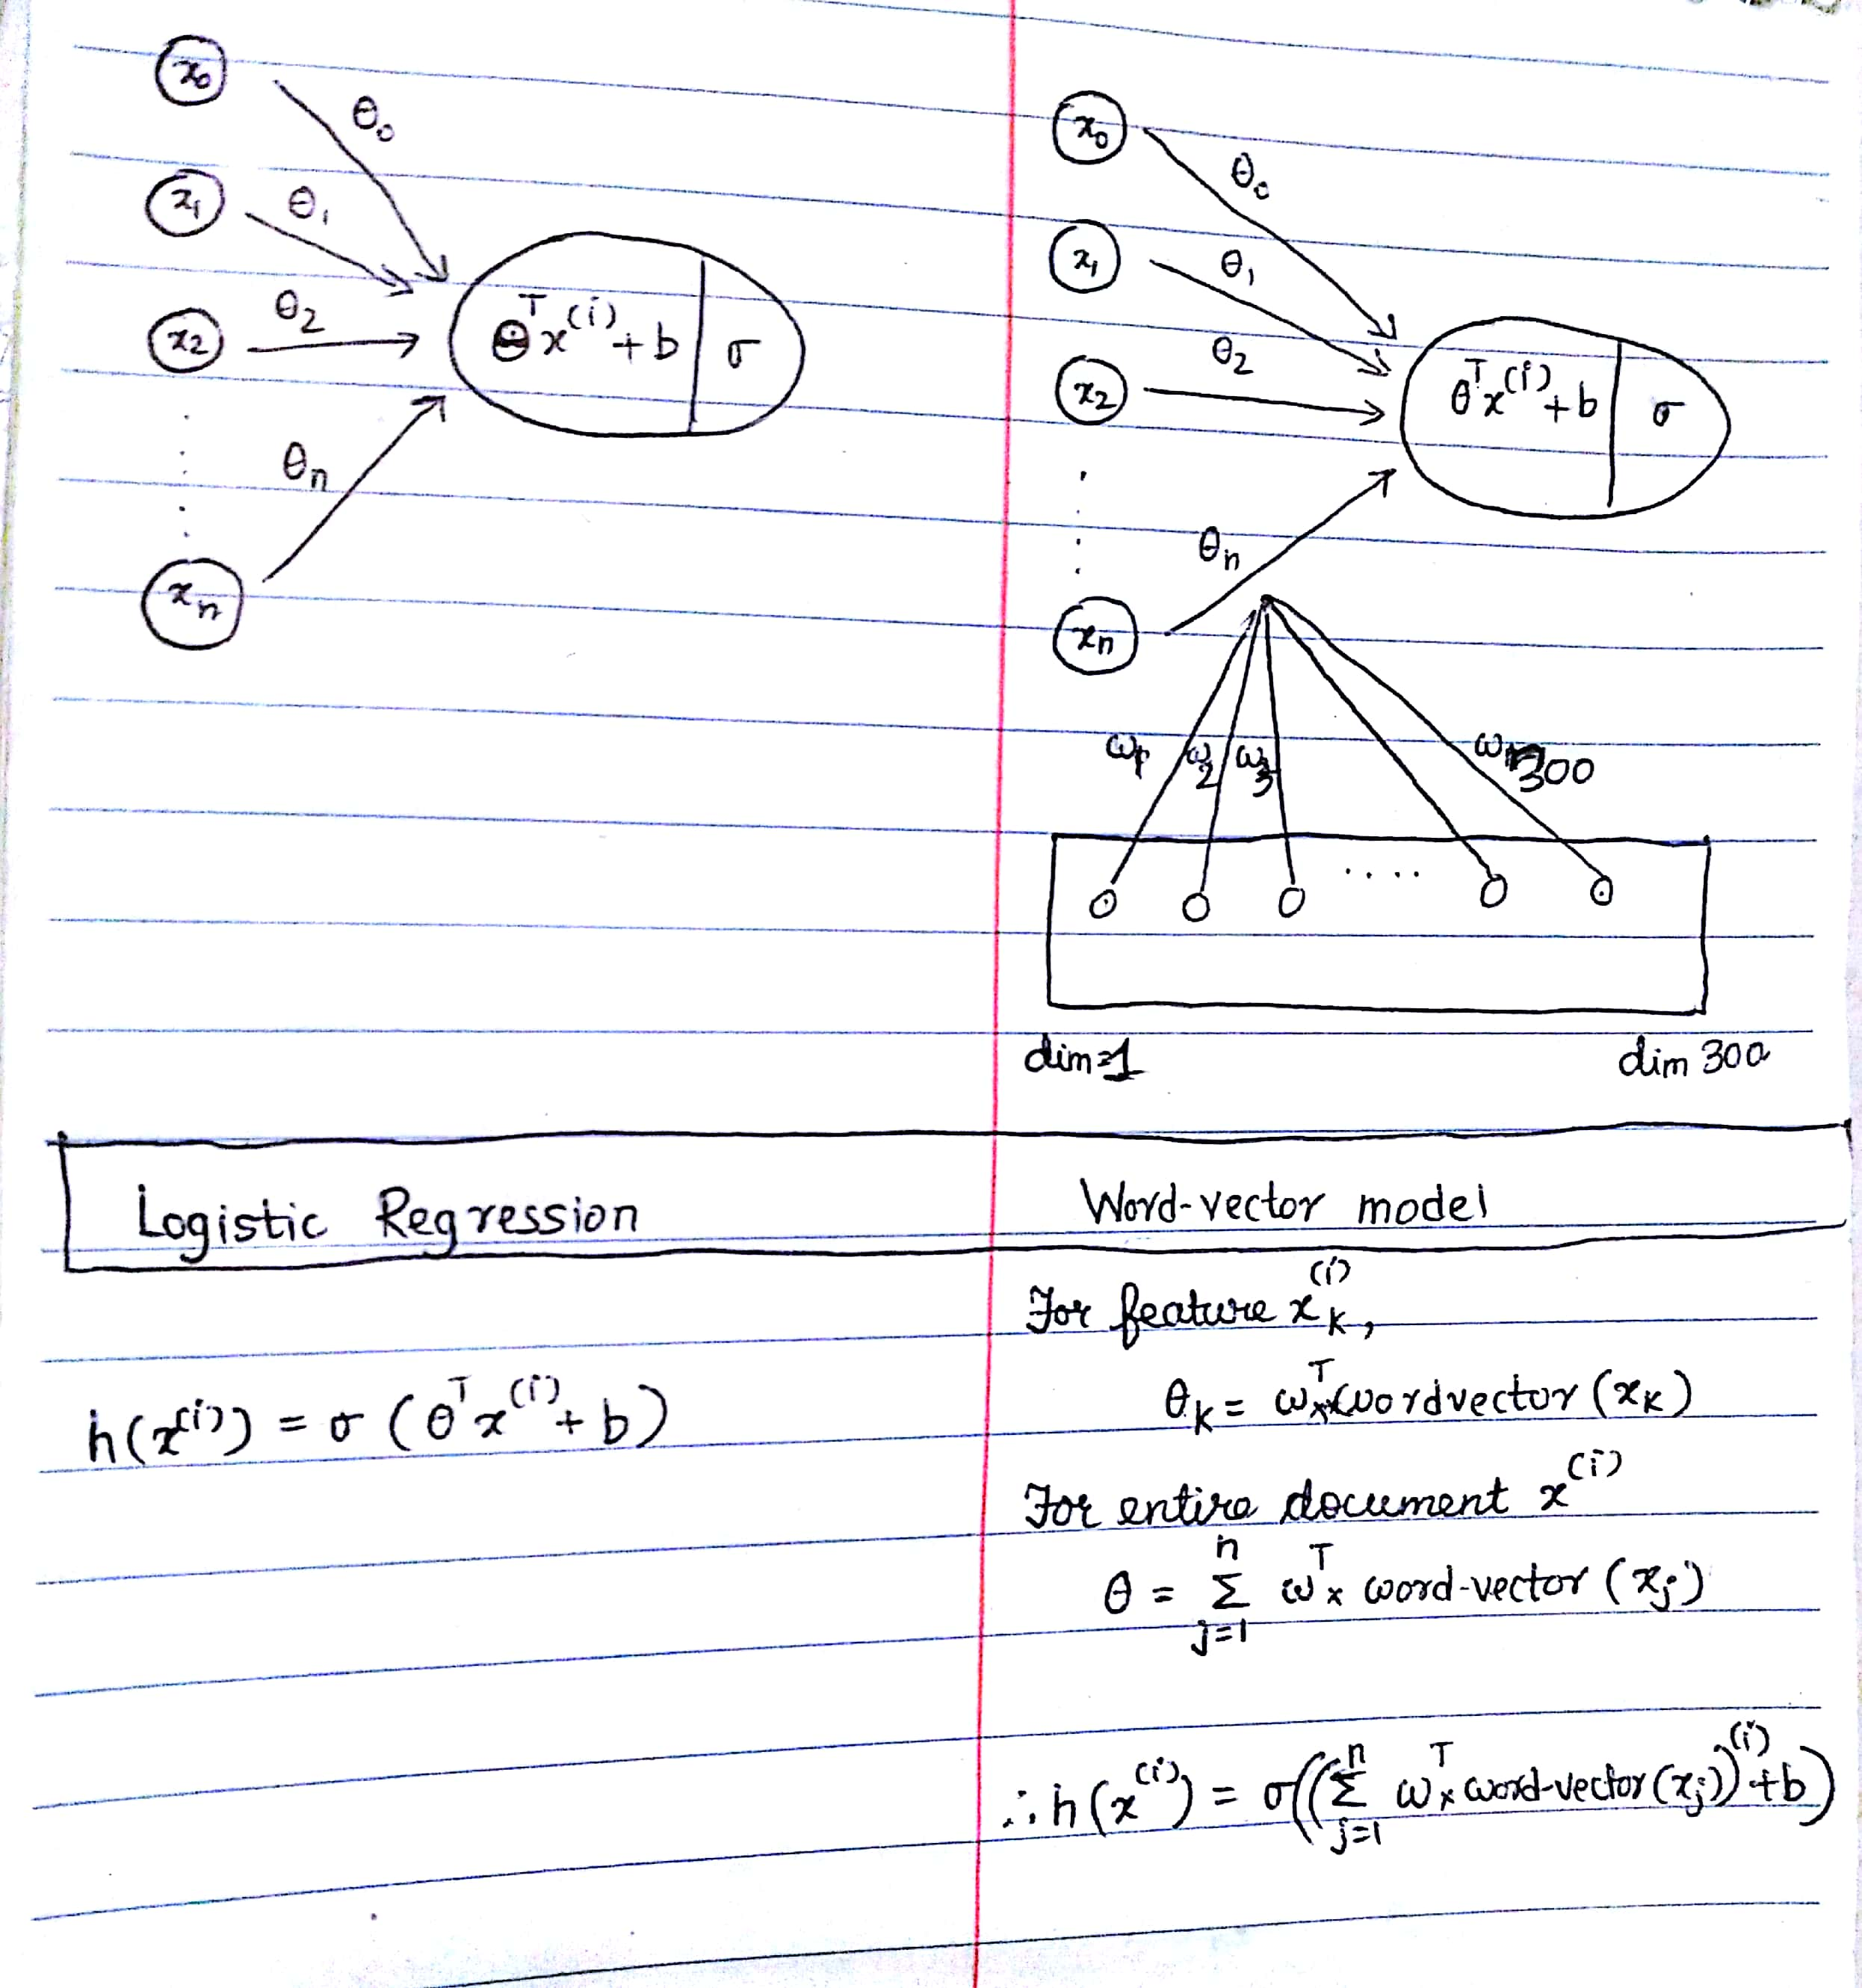
\includegraphics[width=16cm, height=10cm]{wordvec.jpg}\\[1cm]
%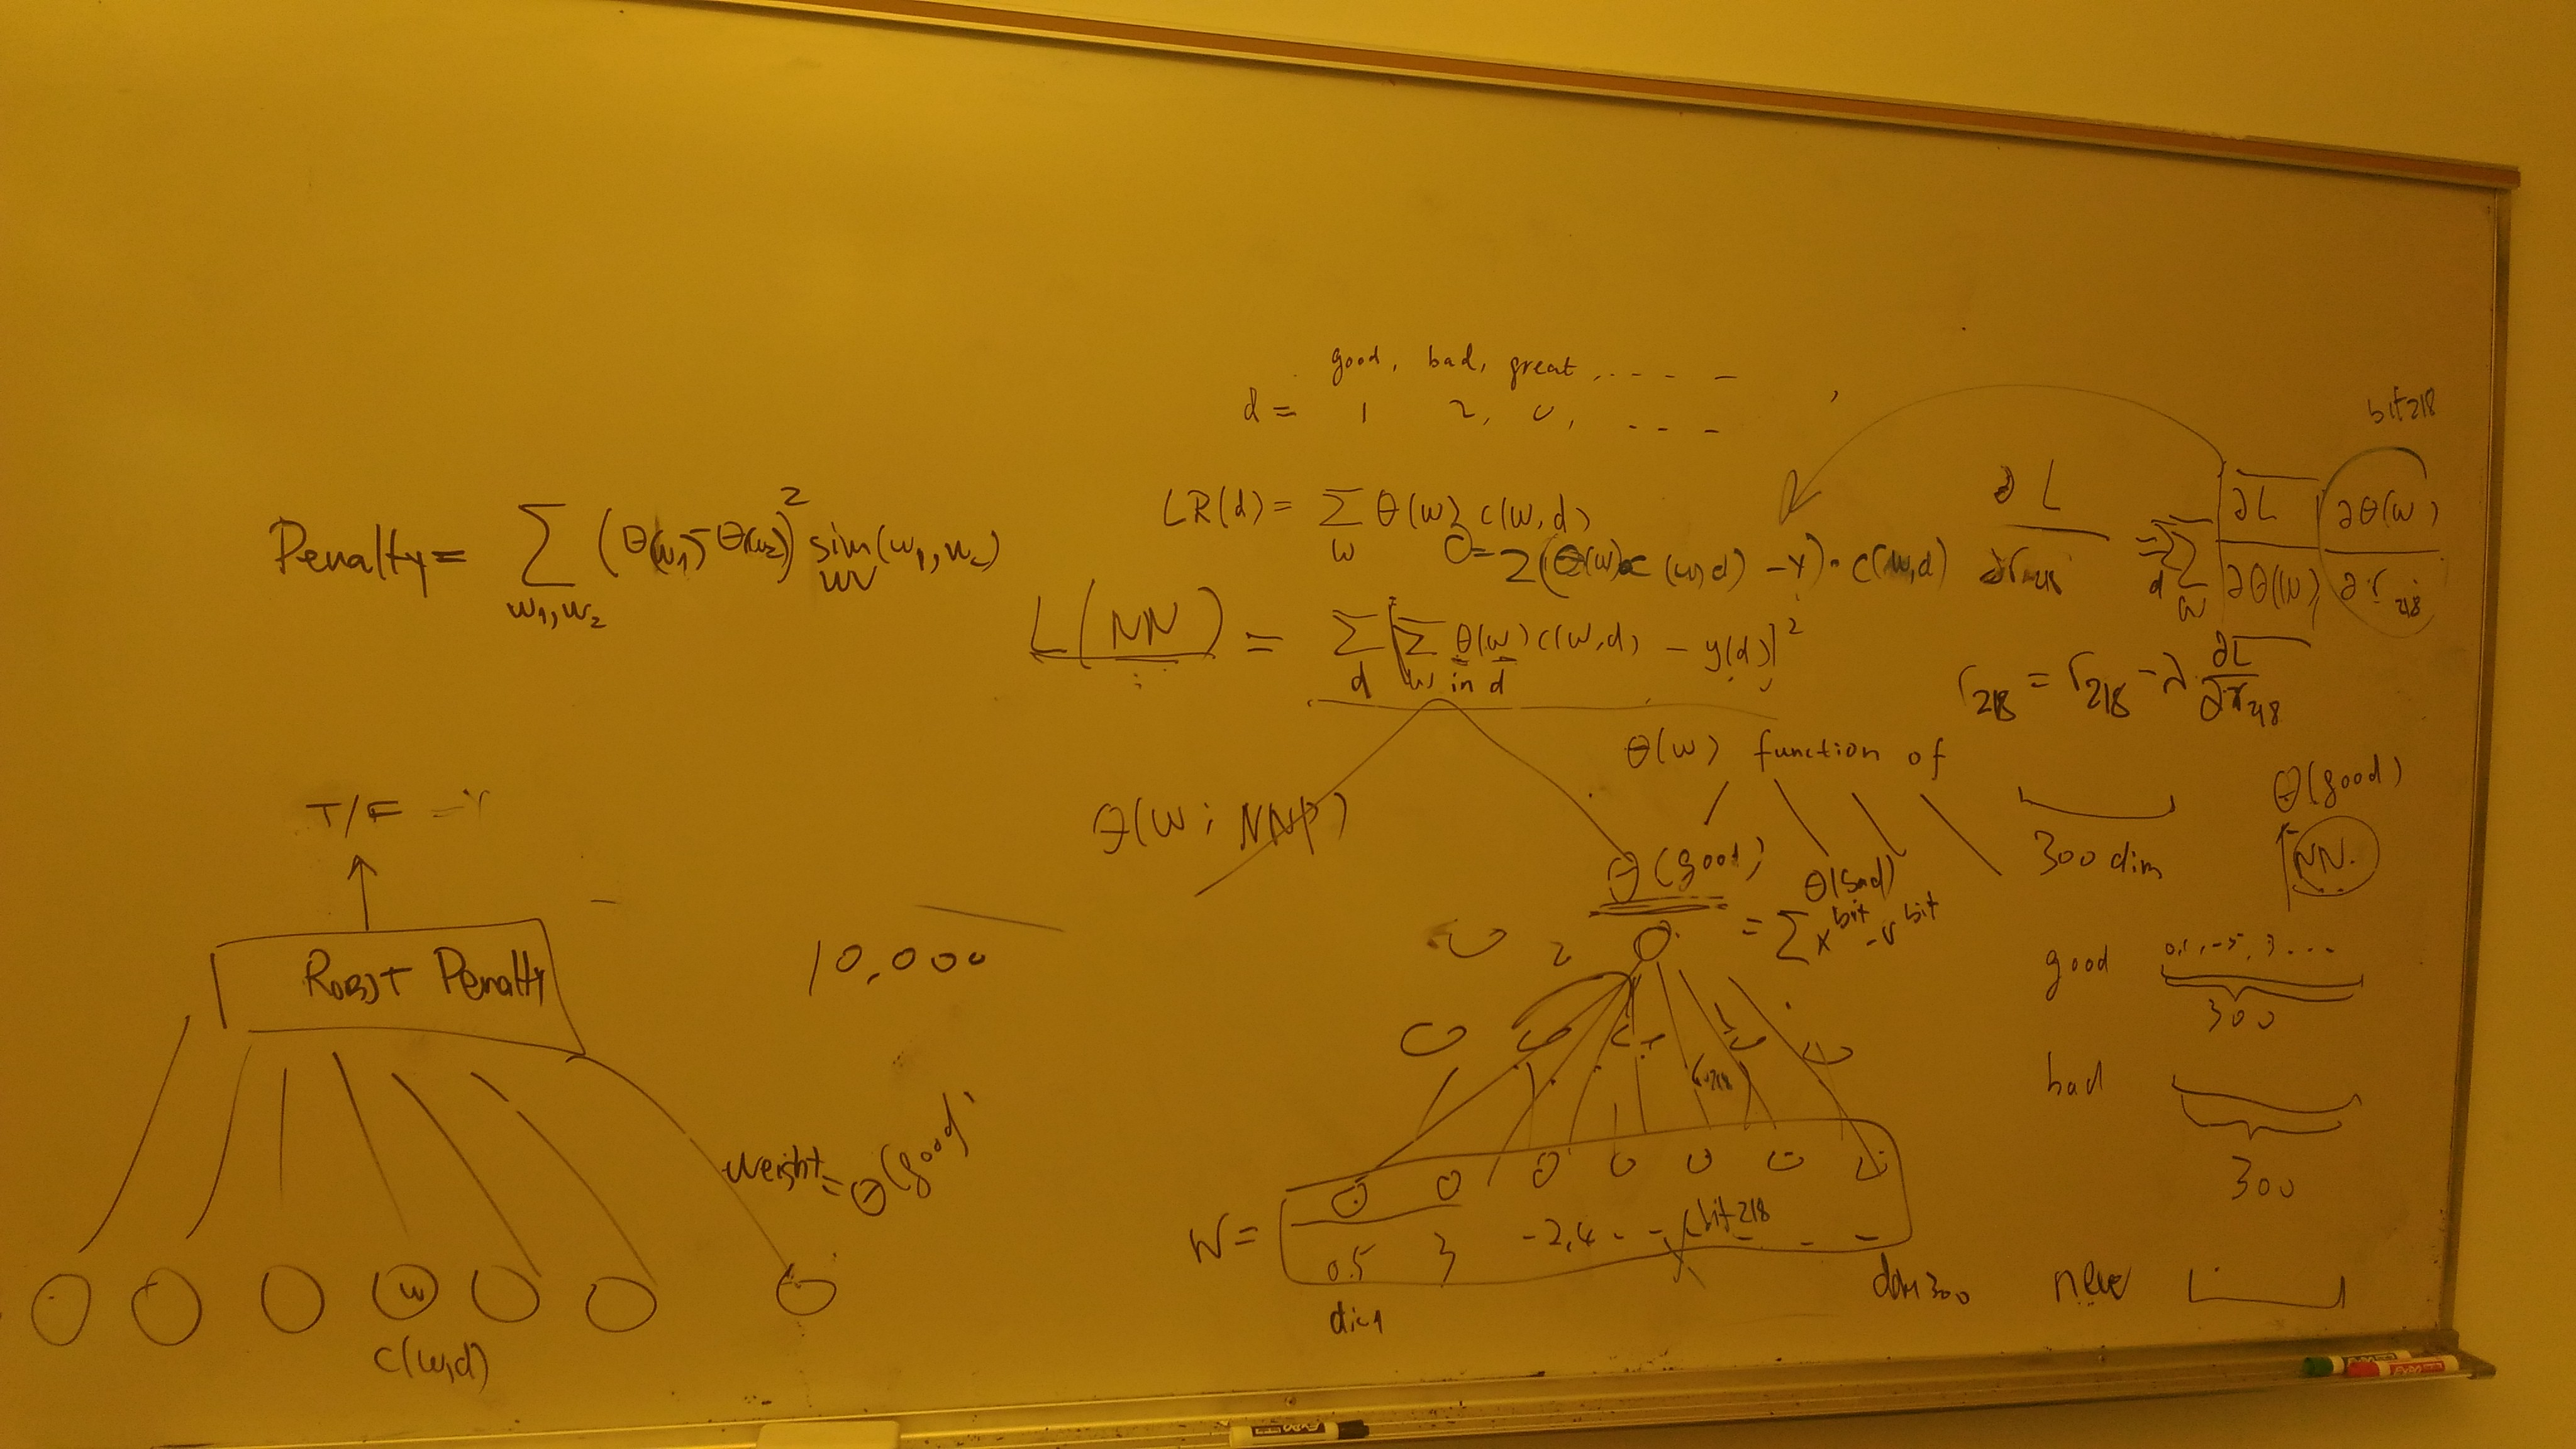
\includegraphics[width=16cm, height=10cm]{cheng.jpg}\\[1cm]

\end{document}